\documentclass[a4paper,12pt]{article}
\usepackage{hyperref}
\usepackage[left=2cm,right=1cm,top=1cm,bottom=1.5cm]{geometry}
\usepackage[utf8]{inputenc}
\usepackage[english,russian]{babel}
\usepackage{graphicx}
\usepackage{amsmath}
\usepackage{amssymb}
\usepackage{cite}
\usepackage{indentfirst}
\usepackage{multicol}
\usepackage{cmap}
\usepackage{array}
\usepackage{varwidth}
\usepackage[T1]{fontenc}



\sloppy

\renewcommand{\baselinestretch}{1.5}

\begin{document}
    \renewcommand{\contentsname}{\Large Содержание}
    \renewcommand{\bibname}{\normalfont\Large\bfseries Список литературы}

    \begin{titlepage}
        \begin{center}
            Министерство науки и высшего образования Российской Федерации \\
            НАЦИОНАЛЬНЫЙ ИССЛЕДОВАТЕЛЬСКИЙ ЯДЕРНЫЙ УНИВЕРСИТЕТ <<МИФИ>> \\*
            \hrulefill
        \end{center}

        \begin{center}
            ИНСТИТУТ ЛАЗЕРНЫХ И ПЛАЗМЕННЫХ ТЕХНОЛОГИЙ\\
            КАФЕДРА №31 ПРИКЛАДНАЯ МАТЕМАТИКА
        \end{center}
        \vspace{1cm}

        \vspace{2em}

        \begin{center}
            \large{ОТЧЕТ}

            по научно-исследовательской работе
            за весенний семестр 2024 года \\

            на тему:
        \end{center}

        \begin{center}
            \large Разработка программного обеспечения для мониторинга здоровья пациентов во время реабилитации

        \end{center}

        \begin{center}
            \large Студент группы Б21-215, Бородин Михаил Сергеевич.
        \end{center}



        \vspace{25em}

        \begin{center}
            г. Москва 2024
        \end{center}
    \end{titlepage}

    \newpage
    \tableofcontents
    \setcounter{page}{3}

    \newpage
    \section*{Аннотация}

    Пациенту, который недавно перенес инфаркт миокарда, требуется контроль за его здоровьем.
    Сейчас для этого ему нужно записываться на прием к врачу, рассказывать обо всех изменениях в самочувствии и симптомах.
    Чтобы избавить врача и пациента от зачастую одинаковых приемов, была придумана методика оценки здоровья человека путем ответа на несложные вопросы в мобильном приложении.

    \newpage

    \section*{Введение}
    \addcontentsline{toc}{section}{Введение}
    \label{sec:4}
    Требуется создать Android/iOS приложение, которым будут пользоваться, как и пациенты, так и врачи.
    У первых должна быть возможность проходить опрос с несложными вопросами об их здоровье, у вторых - просмотр результатов и своевременное уведомление врачей о ключевых изменениях.  \par
    Каждый пациент должен проходить данный опрос раз в две недели.
    Если опрос пройден хорошо, и нет явных признаков ухудшения здоровья, то ему об этом сообщат.
    В противном случае, ему должна высветится надпись: \("\)Скоро Вам позвонит врач,\("\)\, а лечащему врачу придет уведомление об ухудшении здоровья его пациента.
    Таким образом будет происходить контроль за состоянием здоровья человека. \par
    Вредные привычки также играют важную роль в реабилитации.
    Поэтому стоит уведомлениями напоминать пациенту о негативных последствиях данных привычек, а также вести контроль за ними.

    \newpage

    \section{Актуальность}\label{sec:}

    Польза от системы дистанционного наблюдения за пациентами была проанализирована и описана в статье \("\)Study design of Heart failure Events reduction with Remote Monitoring and eHealth Support (HERMeS)\("\)\, 2020. \par
    Люди, подходящие под определенные критерии, были случайным образом разделены на две группы в соотношении 1:1.
    Все пациенты, включенные в исследование, находились под наблюдением в течение 6 месяцев.
    Пациенты, включенные в группу ТМ (Telemedicine group), находились под дистанционным наблюдением и наблюдением в соответствии с конкретным клиническим маршрутом, который включает заранее запланированные структурированные последующие контакты с командой здравоохранения, использующей VC. Пациенты в отделении UC наблюдались в соответствии с UC каждого рекрутингового центра. \par
    Наблюдение и лечение пациентов в отделении ТМ будут основаны на платформе PIRENe. Платформа PIRENe представляет собой комплексное решение для ухода и мониторинга хронических пациентов, смоделированное и протестирован на пациентах с хронической СН.
    Эта платформа позволяет предоставлять многоканальное обслуживание и мониторинг пациентов посредством: \par
    \begin{enumerate}
        \itemМониторинга пациента
        \begin{enumerate}
            \item Биометрические данные (вес, ЧСС и АД);
            \item Отчет о симптомах: семь вопросов, чтобы отразить ухудшение симптомов сердечно-сосудистых заболеваний, в основном ухудшение СН, и один вопрос, чтобы отразить общее ухудшение (см.\ Таблицу~\ref{tab:timesandtenses}).
            Вопросы ставятся так, чтобы ответить «да» или «нет».
        \end{enumerate}
        \item Генерации и управления предупреждающими сигналами, отправляемыми специалистам, закрепленным за каждым пациентом, в случае возникновения одной из следующих ситуаций:
        \begin{enumerate}
            \item Биометрические данные за пределами допустимого диапазона.
            \item Любой тревожный симптом среди ответов на анкету (один ответ «да» в анкете генерирует предупреждающий сигнал в платформе).
            \item Отсутствие биометрических измерений в любой день
        \end{enumerate}
        \item Последующее наблюдение посредством телеконсультаций (видеоконференция, аудиоконференция, рассылка по почте и управление входящими и исходящими звонками) между специалистами и пациентами/опекунами.
    \end{enumerate}

    \begin{table}[h]
        \caption{Вопросы, на которые отвечали пациенты.}
        \label{tab:timesandtenses}
        \begin{center}
            \begin{tabular}{|V{10cm}|c|}
                \hline
                Вопрос & Ответ \\
                \hline
                Мои ноги опухли больше, чем обычно & Да/Нет \\
                \hline
                Я чувствую себя более утомленным, уставшим или с ощущением удушья.
                & Да/Нет \\
                \hline
                У плохо спал из-за одышки или ощущения удушья.
                & Да/Нет \\
                \hline
                Мне нужно было больше подушек, чтобы лучше дышать ночью, лежа на кровати.
                & Да/Нет \\
                \hline
                Мне приходилось спать сидя из-за одышки или ощущения удушья, когда я лежал на кровати.
                & Да/Нет \\
                \hline
                Я чувствовал слабость и головокружение сильнее, чем обычно.
                & Да/Нет \\
                \hline
                У меня сильнее болела грудь, чем обычно.
                & Да/Нет \\
                \hline
                В общем, я чувствую себя хуже, чем обычно.
                & Да/Нет \\
                \hline
            \end{tabular}
        \end{center}
    \end{table}

    Проведенные исследования показали, что данная стратегия предоставления управляемой помощи, приведет к значительному снижению смертности или повторной госпитализации у этих пациентов высокого риска в \("\)уязвимой фазе\("\) заболевания.


    \newpage
    \section{Структура опросов}\label{sec:-}

    \subsection{Основной опрос}\label{subsec:-}

    Опрос представляет собой дерево.
    В зависимости от данного человеком ответа, будет подбираться следующий вопрос.
    Вопросы разбиваются на блоки.
    Каждый ответ на вопрос имеет свою ценность в виде баллов.
    Если при ответе на вопросы пациент набрал N-ное количество баллов и более для данного блока, то это означает, что его здоровье ухудшилось и стоит обратиться к врачу.

    \begin{figure}[h]
        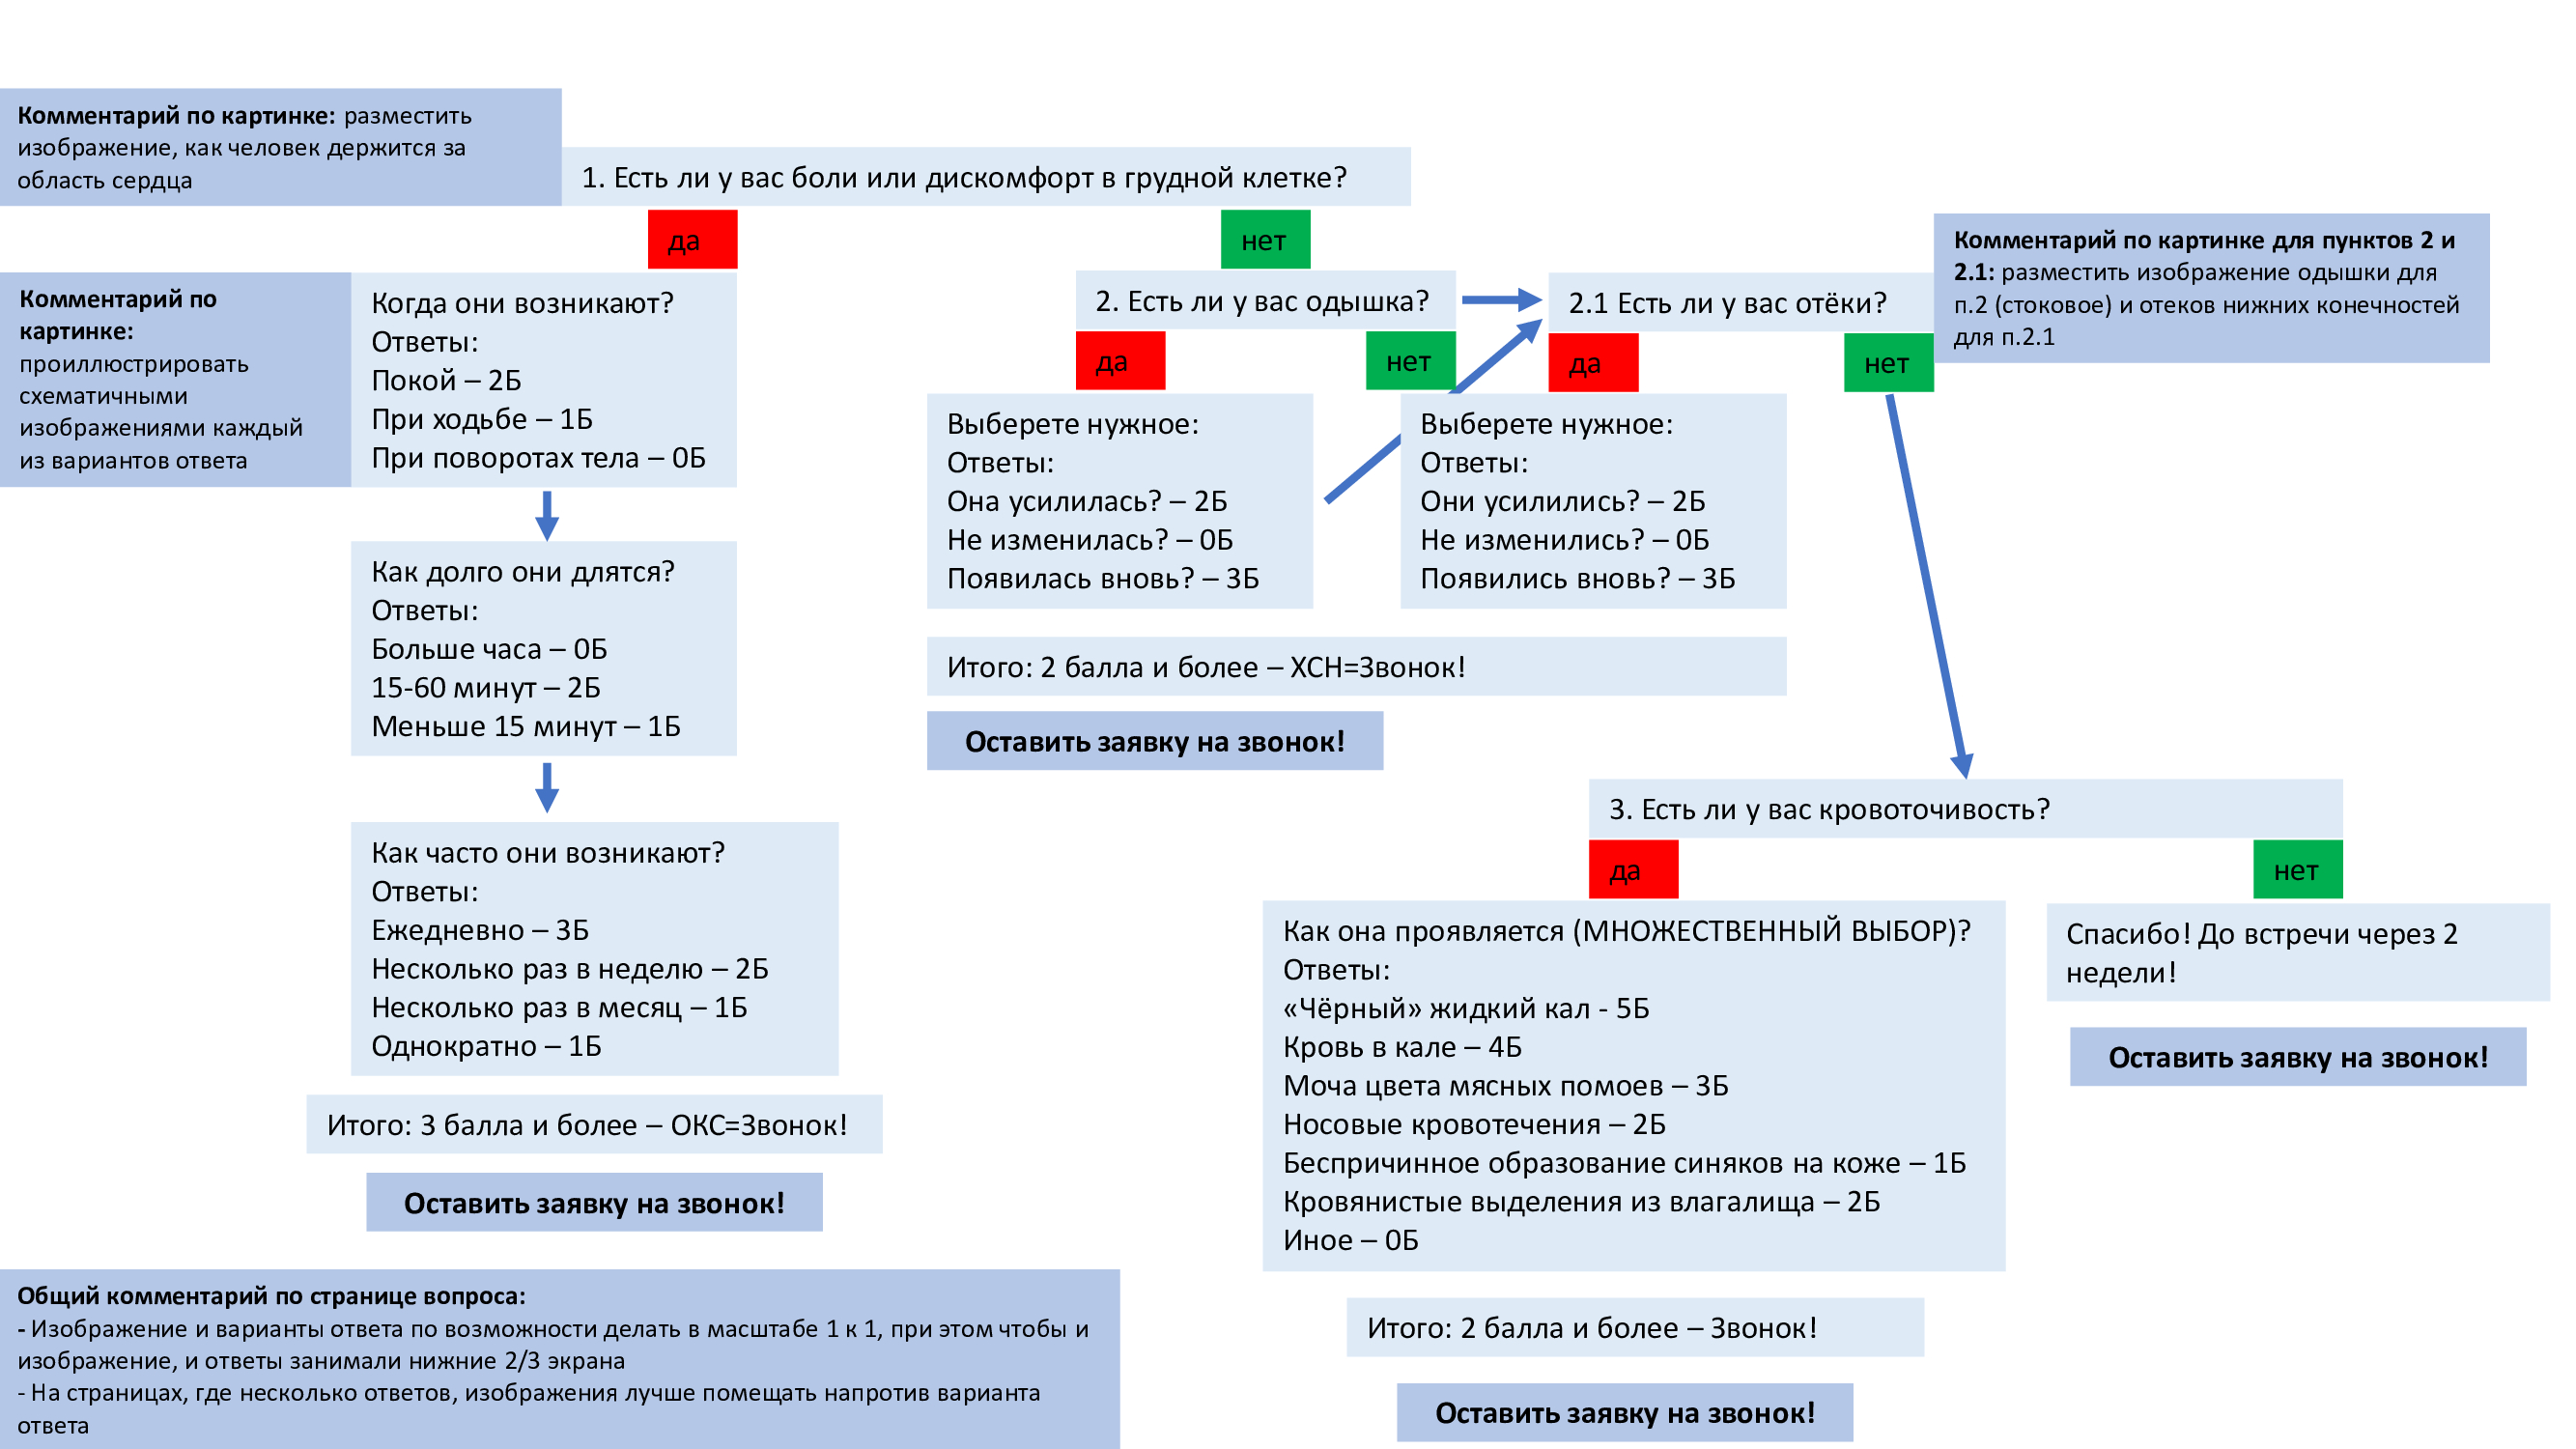
\includegraphics[scale=0.175]{images/presentation/1cbc101521d4d97c799189ce193d279d-0}
        \caption{Структура опроса.}\label{fig:figure}
    \end{figure}

    К примеру, первым вопросом будет \("\)Есть ли у вас боли или дискомфорт в грудной клетке?
    .
    При положительном ответе, пациент попадает в блок вопросов, состоящий из 3-х вопросов.
    При наборе трех и более баллов за эти 3 вопроса, потребуется консультация с врачом.
    В противном случае, консультация на данном этапе не требуется. \par
    Если на первый вопрос был дан ответ \("\)Нет,\("\)\, то выдается следующий вопрос, ответ на который определит, показывать вопросы из нового блока, или перейти к следующему.

    \subsection{Контроль за приемом лекарств}\label{subsec:---}

    Не менее важно контролировать прием всех прописанных лекарств.
    Отвечая на вопросы, можно определить, какие из них пациент не принимает, а также узнать саму причину.
    Можно определить, какое лекарство вызывает у человека ту или иную реакцию в организме.
    Проходить данный опрос предлагается раз в 3 месяца.

    \begin{figure}[h]
        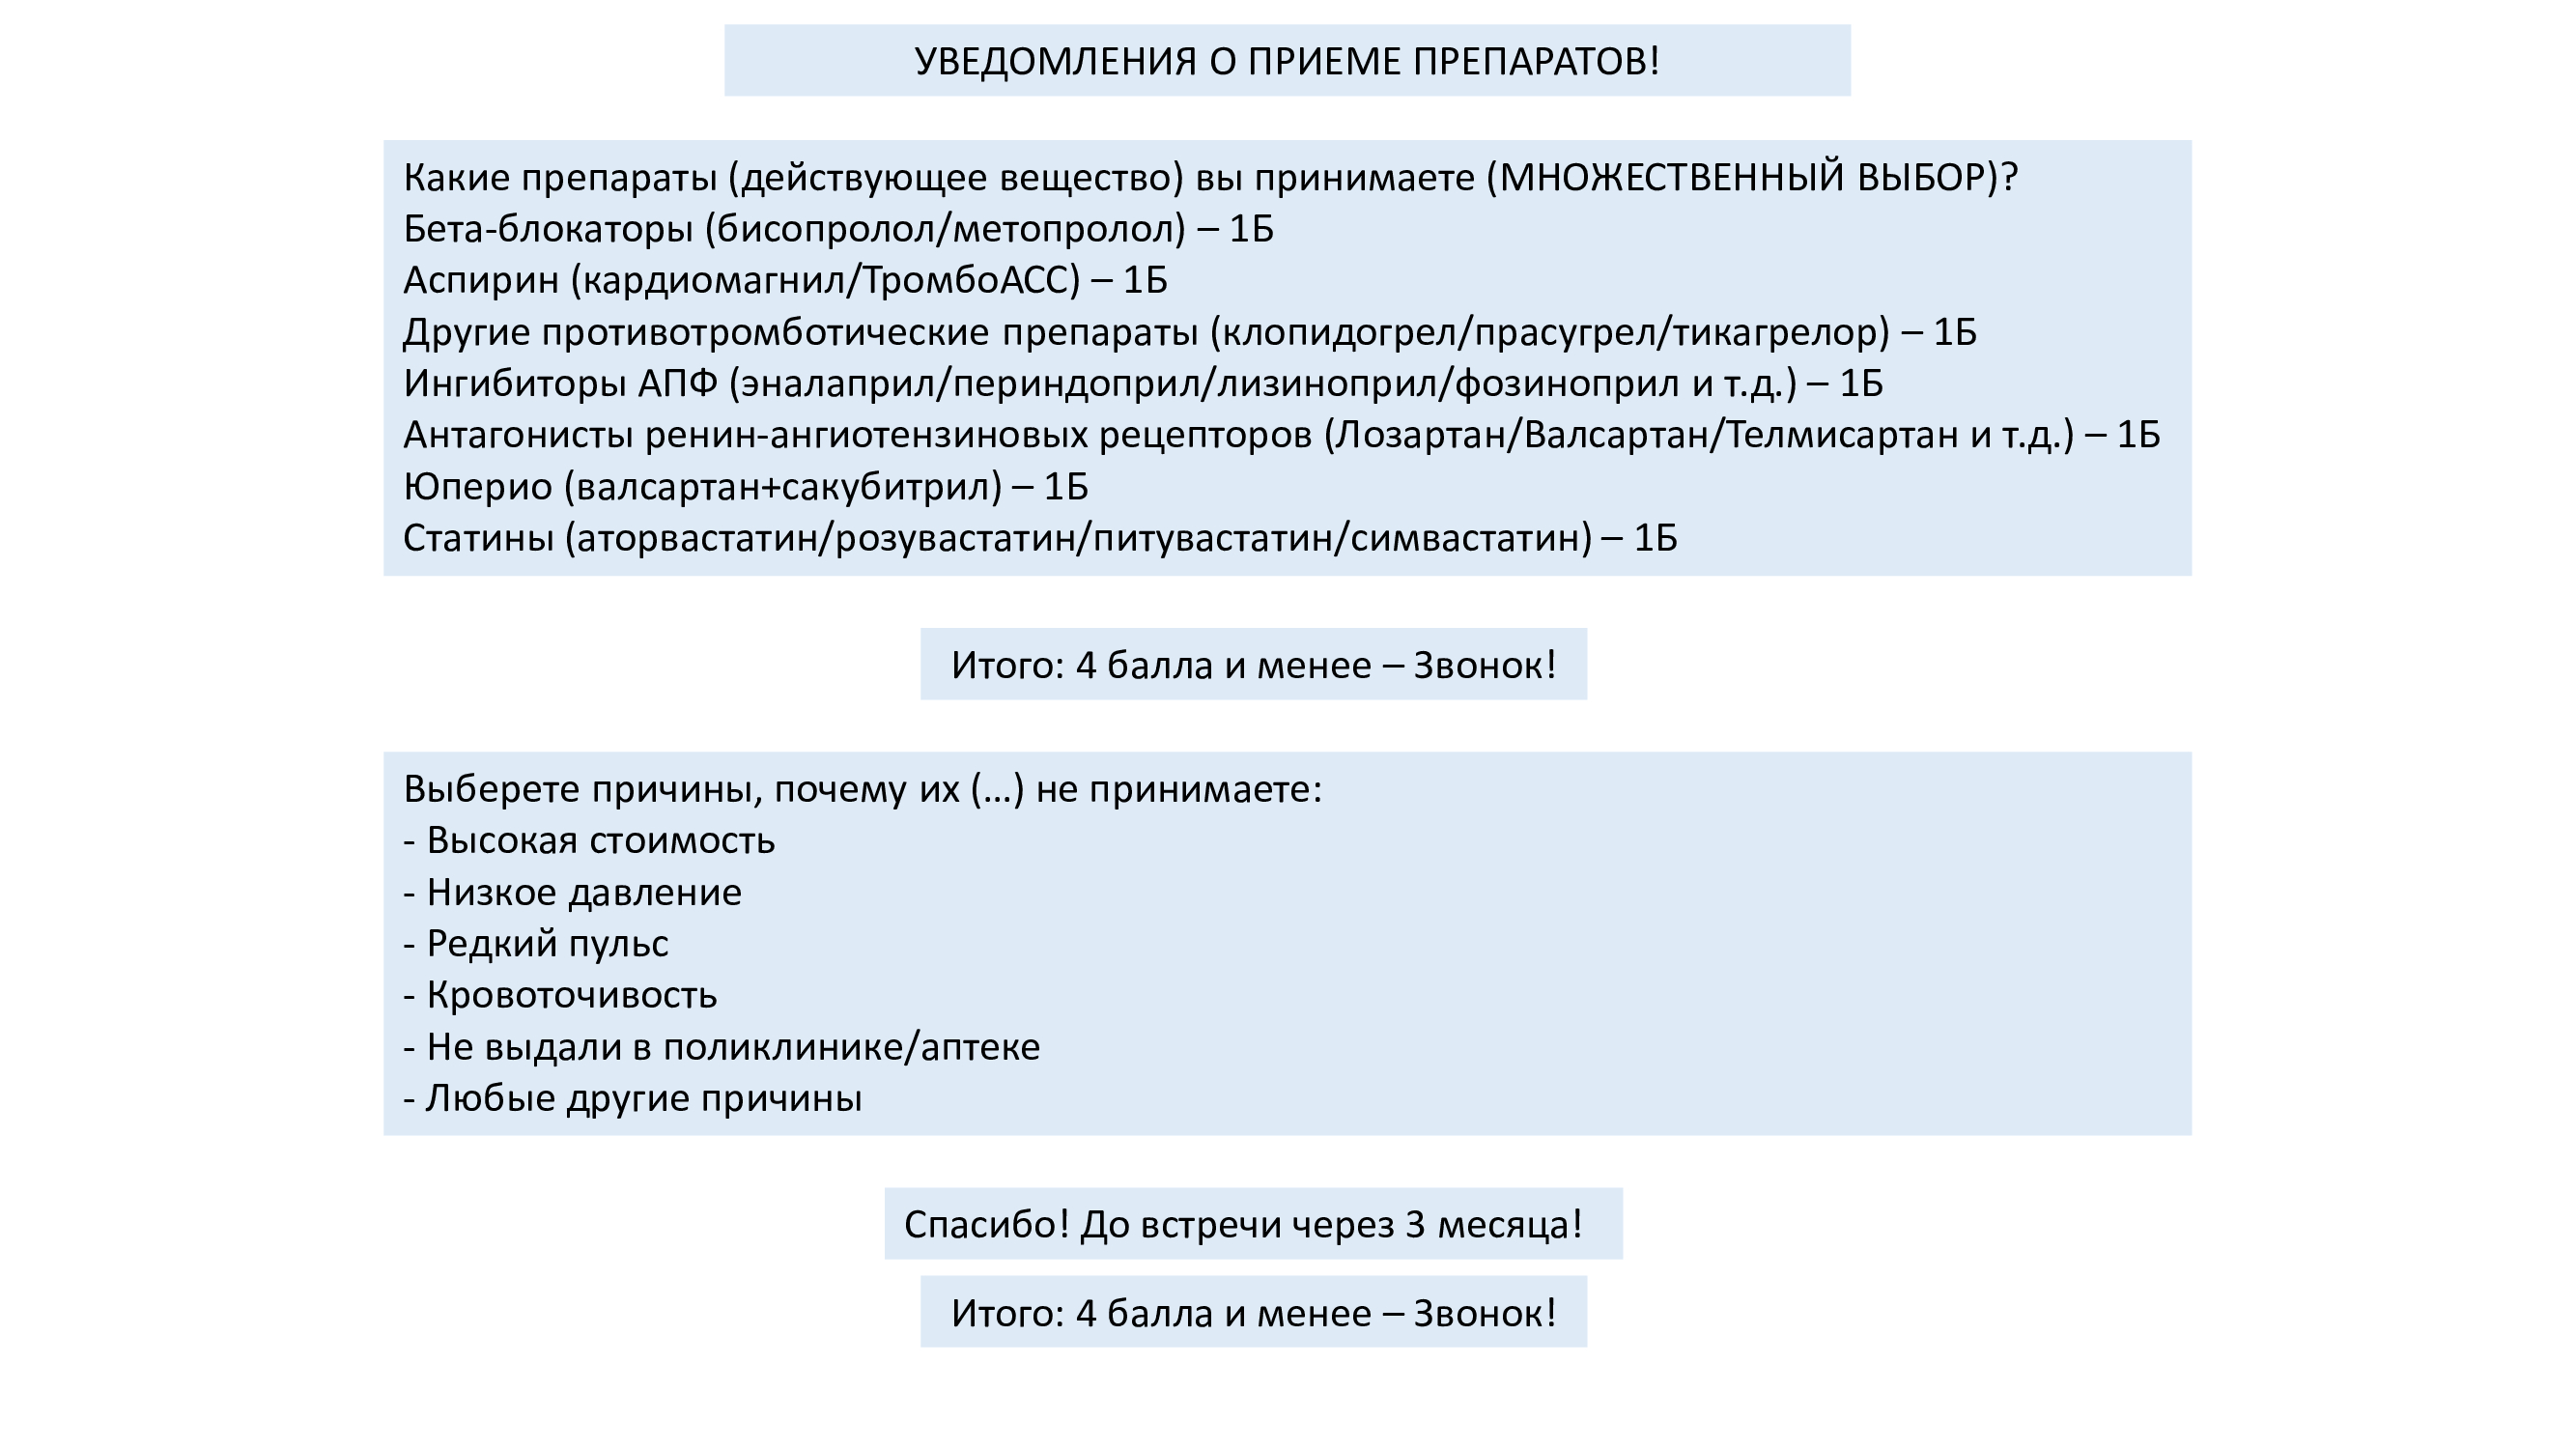
\includegraphics[scale=0.175]{images/presentation/1cbc101521d4d97c799189ce193d279d-1}
        \caption{Опрос лекарства.}\label{fig:figure2}
    \end{figure}

    \newpage

    \subsection{Вредные привычки и физическая активность}\label{subsec:----}

    Раз в полгода стоит напоминать пациенту о важности соблюдения режима, о вреде всех его привычек.
    Данный опрос предназначен для этого.

    \begin{figure}[h]
        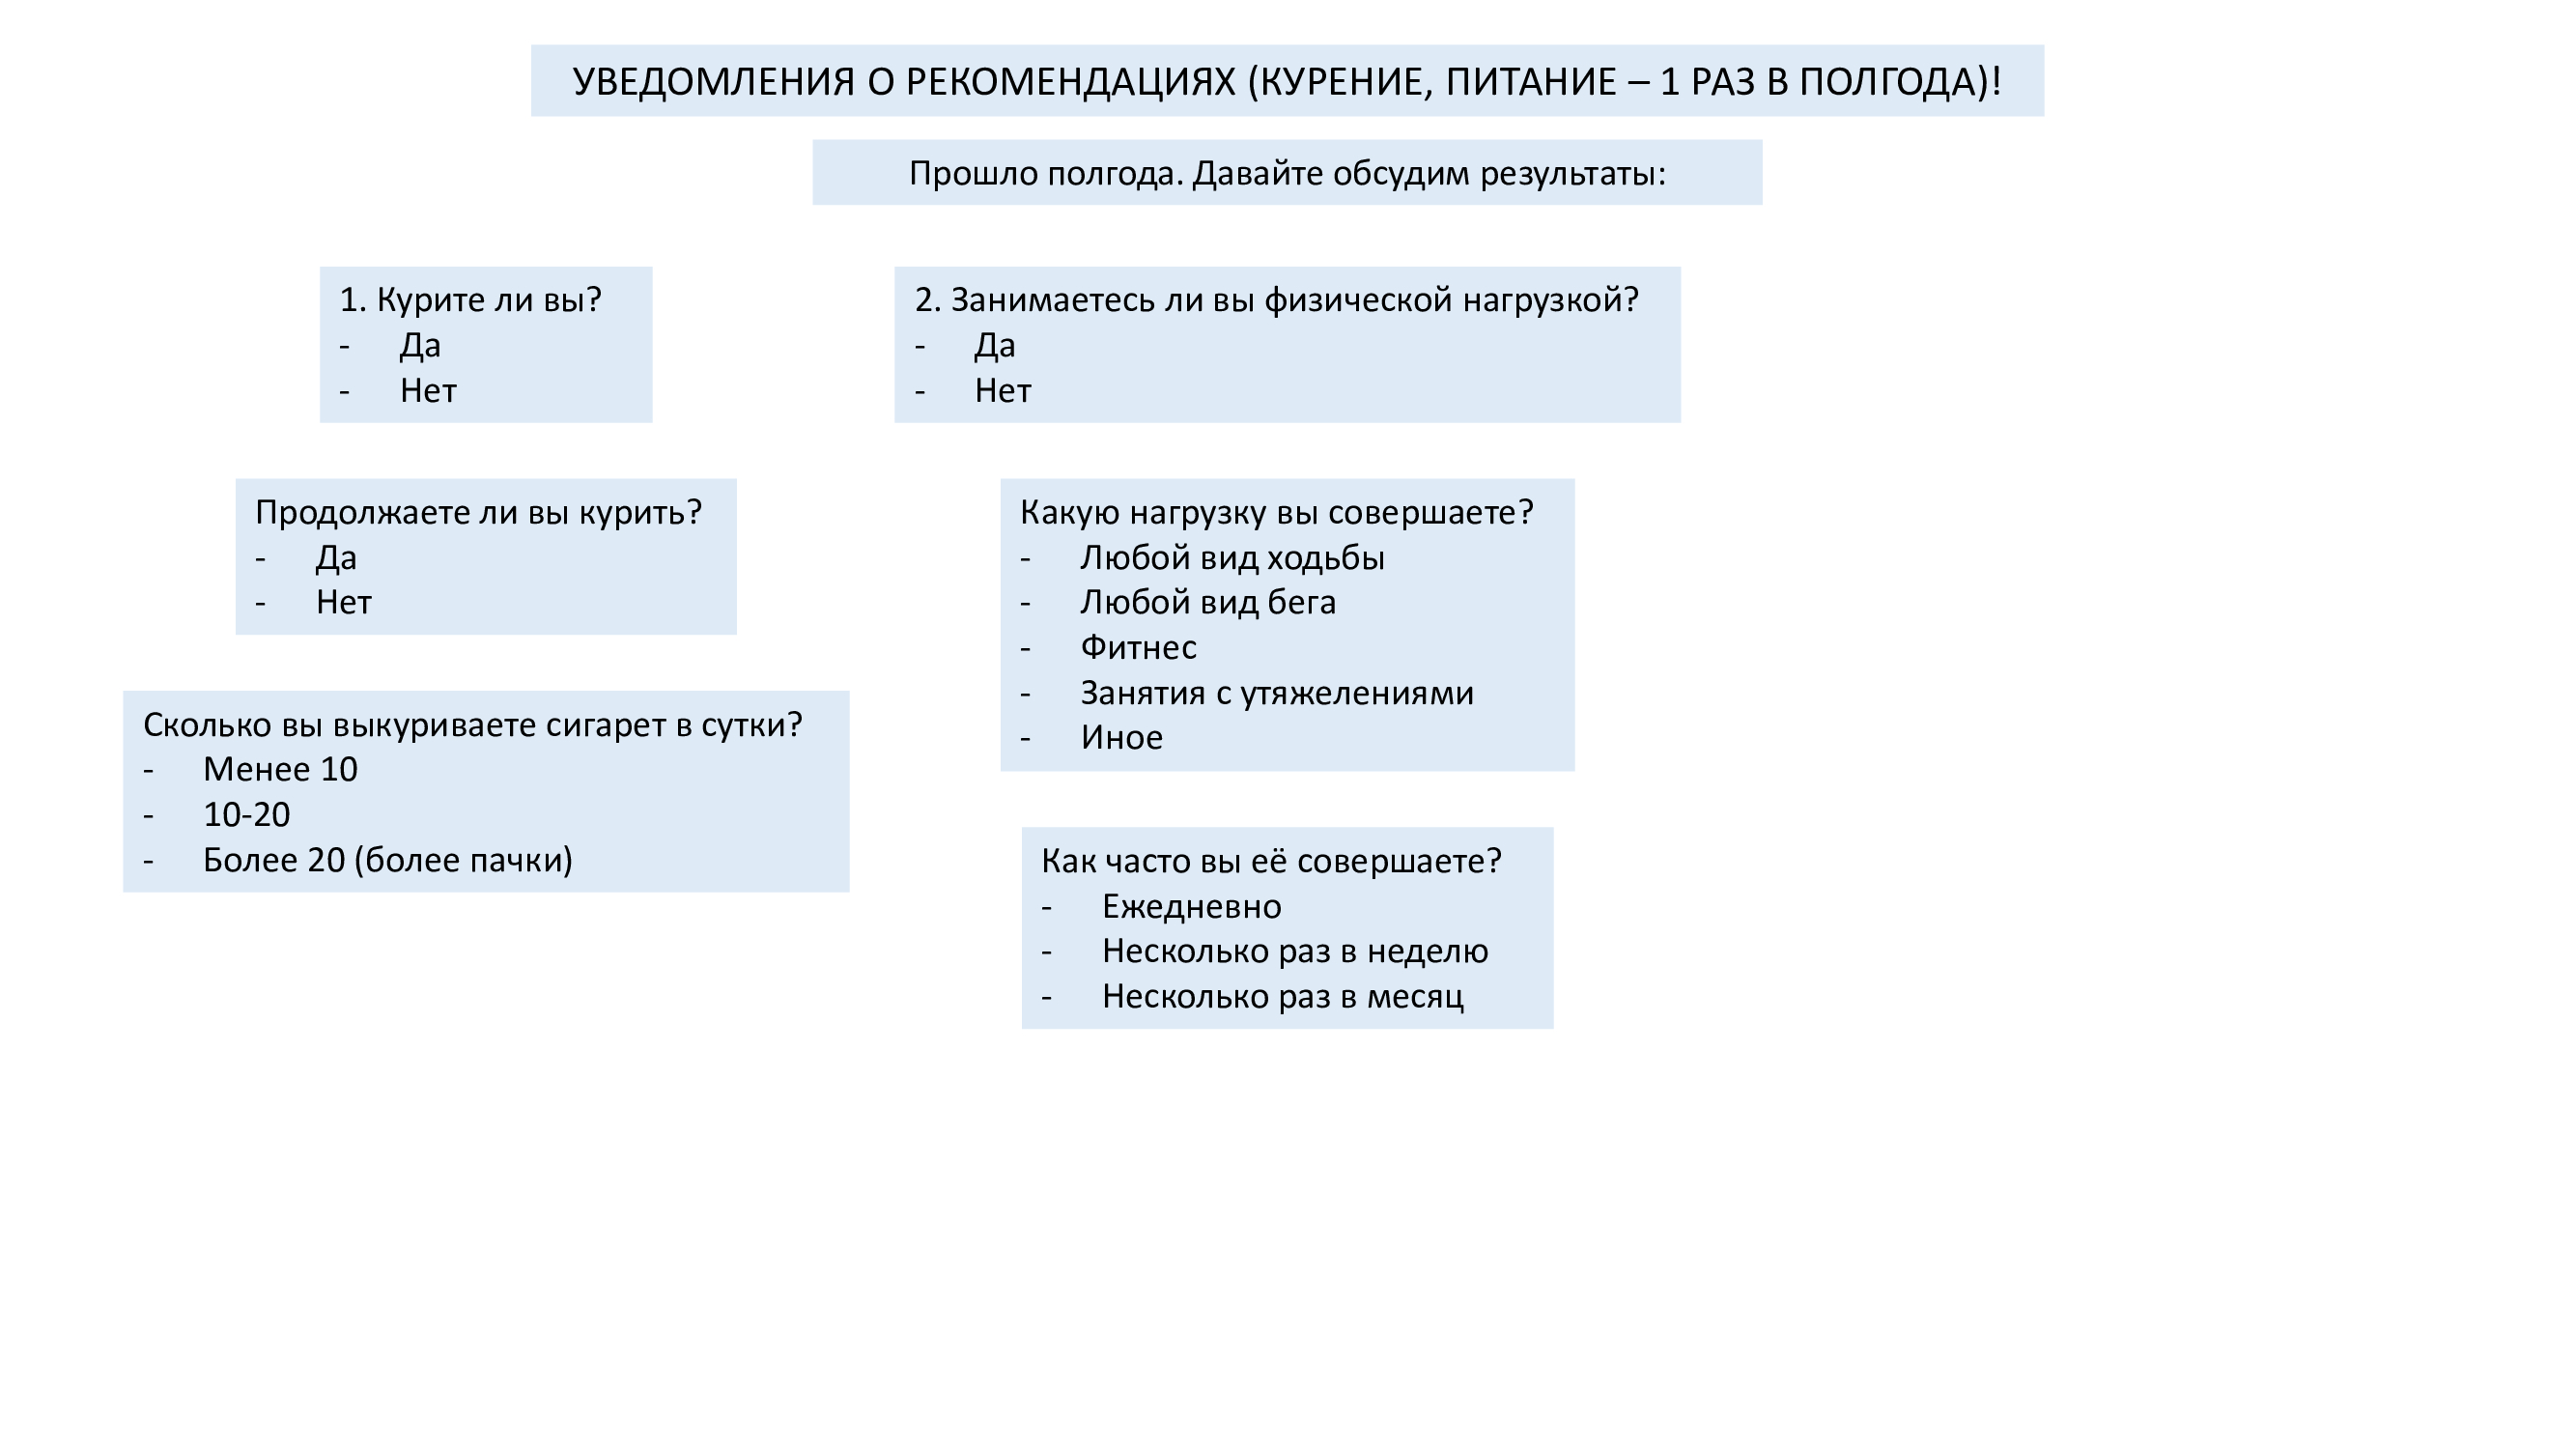
\includegraphics[scale=0.175]{images/presentation/1cbc101521d4d97c799189ce193d279d-2}
        \caption{Рекомендации.}\label{fig:figure3}
    \end{figure}


    \newpage
    \section{Задачи}\label{sec:2}
    Проект разделен на 3 зоны ответственности:
    \begin{enumerate}
        \item Серверная часть
        \item Мобильное приложение для пациентов, в нем они приходят опросы и взаимодействуют с нашим сервисом.
        Так же им приходят уведомления о необходимости прохождения опроса или взаимодействия с врачом.
        \item Веб-сайт для врачей, в нем они смотрят результаты опросов пациентов и прочую статистику.
    \end{enumerate}
    Я ответственен за веб-приложение для врачей.
    Передо мной были поставлены такие задачи:


    \begin{enumerate}
        \item Выбор фреймворка.
        \item Постановка задач, которые должны быть реализованы в коде.
        \item Выбор необходимых технологий и причины почему именно эту технологию нужно использовать.
        \item Написание кода.
        \item Написание документации к существующему коду.

    \end{enumerate}

    \newpage
    \section{Выбор фреймворка и технологий}\label{sec:---}
    ReactJS:
    \begin{enumerate}
        \item Популярность и Сообщество: React является одной из самых популярных библиотек для разработки пользовательских интерфейсов.
        Он поддерживается Facebook и имеет огромное сообщество разработчиков, что облегчает поиск решений на возникающие вопросы и проблемы.

        \item Компонентный подход: React использует компонентную архитектуру, что упрощает разработку и поддержку сложных пользовательских интерфейсов.
        Компоненты можно переиспользовать в разных частях приложения, что способствует более чистому и организованному коду.

        \item Высокая производительность: React эффективно обновляет и рендерит только те компоненты, которые изменились, благодаря виртуальному DOM\@.
        Это обеспечивает высокую производительность приложения даже при сложных интерфейсах.

        \item Экосистема и инструменты: React имеет обширную экосистему библиотек и инструментов, включая React Router для маршрутизации и Redux для управления состоянием, что позволяет строить приложения любой сложности.

    \end{enumerate}


    Vite:
    \begin{enumerate}
        \item Быстрая разработка: Vite был создан для того, чтобы обеспечить быстрый старт и быструю разработку.
        Он использует современную архитектуру, которая минимизирует время загрузки и время перезапуска сервера разработки.


        \item Модульная система: Vite использует нативные ES-модули в браузере для разработки, что исключает необходимость в тяжелых бандлах и позволяет быстрее обновлять модули.

        \item Оптимизация сборки: Vite обеспечивает быструю и оптимизированную сборку благодаря Rollup, что позволяет создавать высокопроизводительные производственные сборки.

        \item Совместимость: Vite поддерживает множество фреймворков и библиотек, включая React, что делает его гибким и универсальным инструментом для разработки современных веб-приложений.

    \end{enumerate}


    Material-UI
    \begin{enumerate}
        \item Компоненты высокого качества: Material-UI предоставляет набор готовых к использованию компонентов, соответствующих принципам Material Design от Google.
        Это позволяет быстро создавать привлекательные и функциональные пользовательские интерфейсы.

        \item Настраиваемость: Все компоненты Material-UI легко настраиваются под конкретные потребности проекта.
        Можно изменять темы, стили и поведение компонентов, чтобы они соответствовали дизайну приложения.

        \item Поддержка и документация: Material-UI имеет отличную документацию и большую базу примеров, что облегчает процесс обучения и внедрения в проект.

        \item Совместимость с React: Material-UI разработан специально для использования с React, что обеспечивает бесшовную интеграцию и улучшает разработку интерфейсов на React.

    \end{enumerate}

    \newpage
    \section{Веб-приложение}\label{sec:-2}

    \subsection{Аутентификация}\label{subsec:}
    Стартовая страница.
    На ней происходит аутентификация врача.
    \begin{figure}[h]
        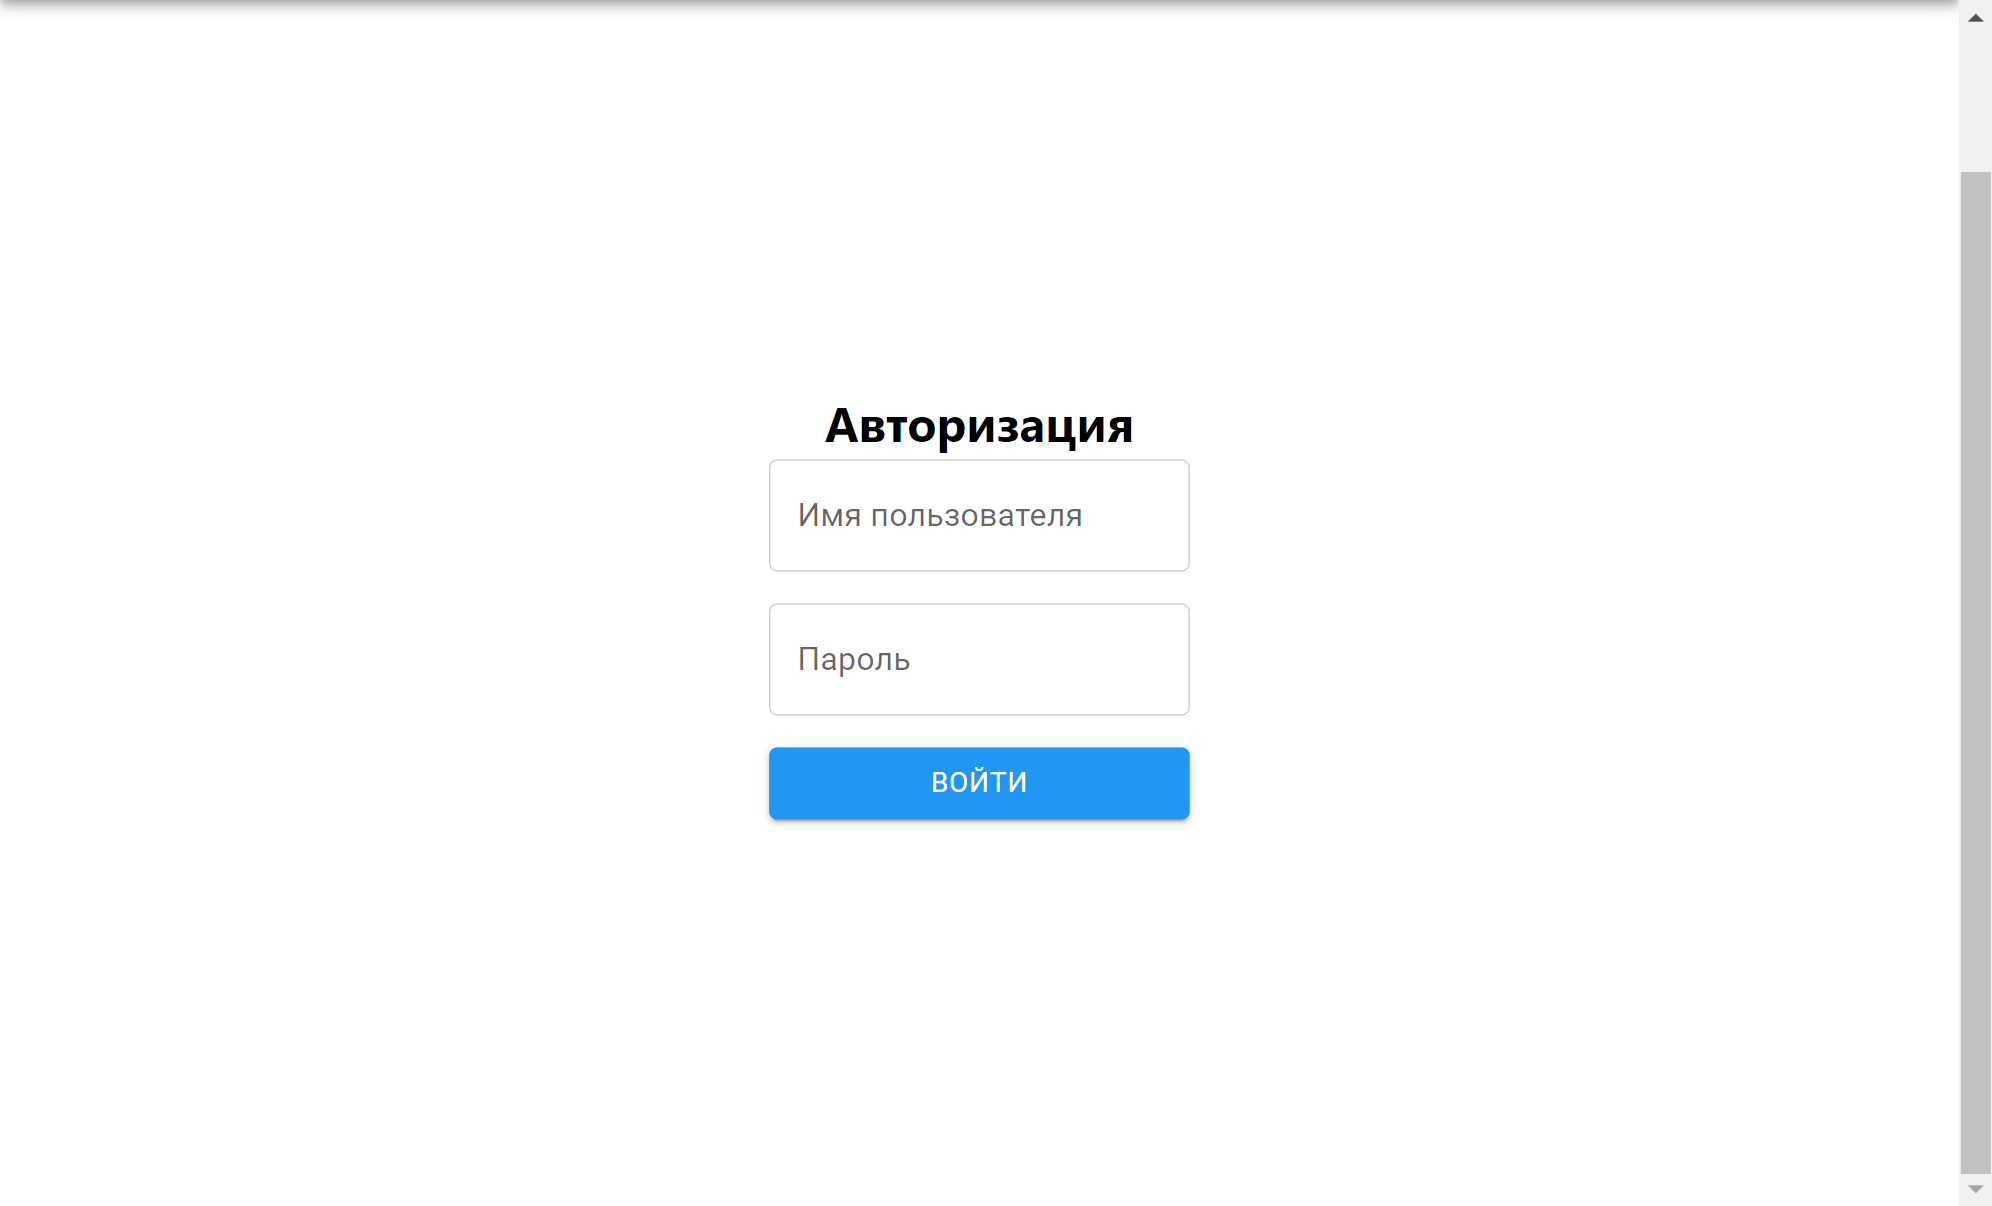
\includegraphics[scale=0.25]{images/screenshots/auth}
        \caption{Аутентификация.}\label{fig:figure4}
    \end{figure}

    \subsection{Главная страница}\label{subsec:-2}
    На главной странице уже появляется хэдер, который есть во всем приложении, кроме страницы аутентификации.
    В нем есть ссылки на саму главную страницу, на страницу регистрации пациента, так же имя врача, ссылка на его персональную страницу и возможность выхода из аккаунта.
    В основном окне представлена таблица с результатами последних опросов, которые прошли пациенты.
    В каждой строке нам важно знать, в какое время это произошло, с кем конкретно.
    Важная графа с оценкой результатов опроса, она меняет свой цвет в зависимости от результата, чтобы врач мог сразу выделить отрицательные результаты и приступать к дальнейшим действиям.
    \begin{figure}[ht]
        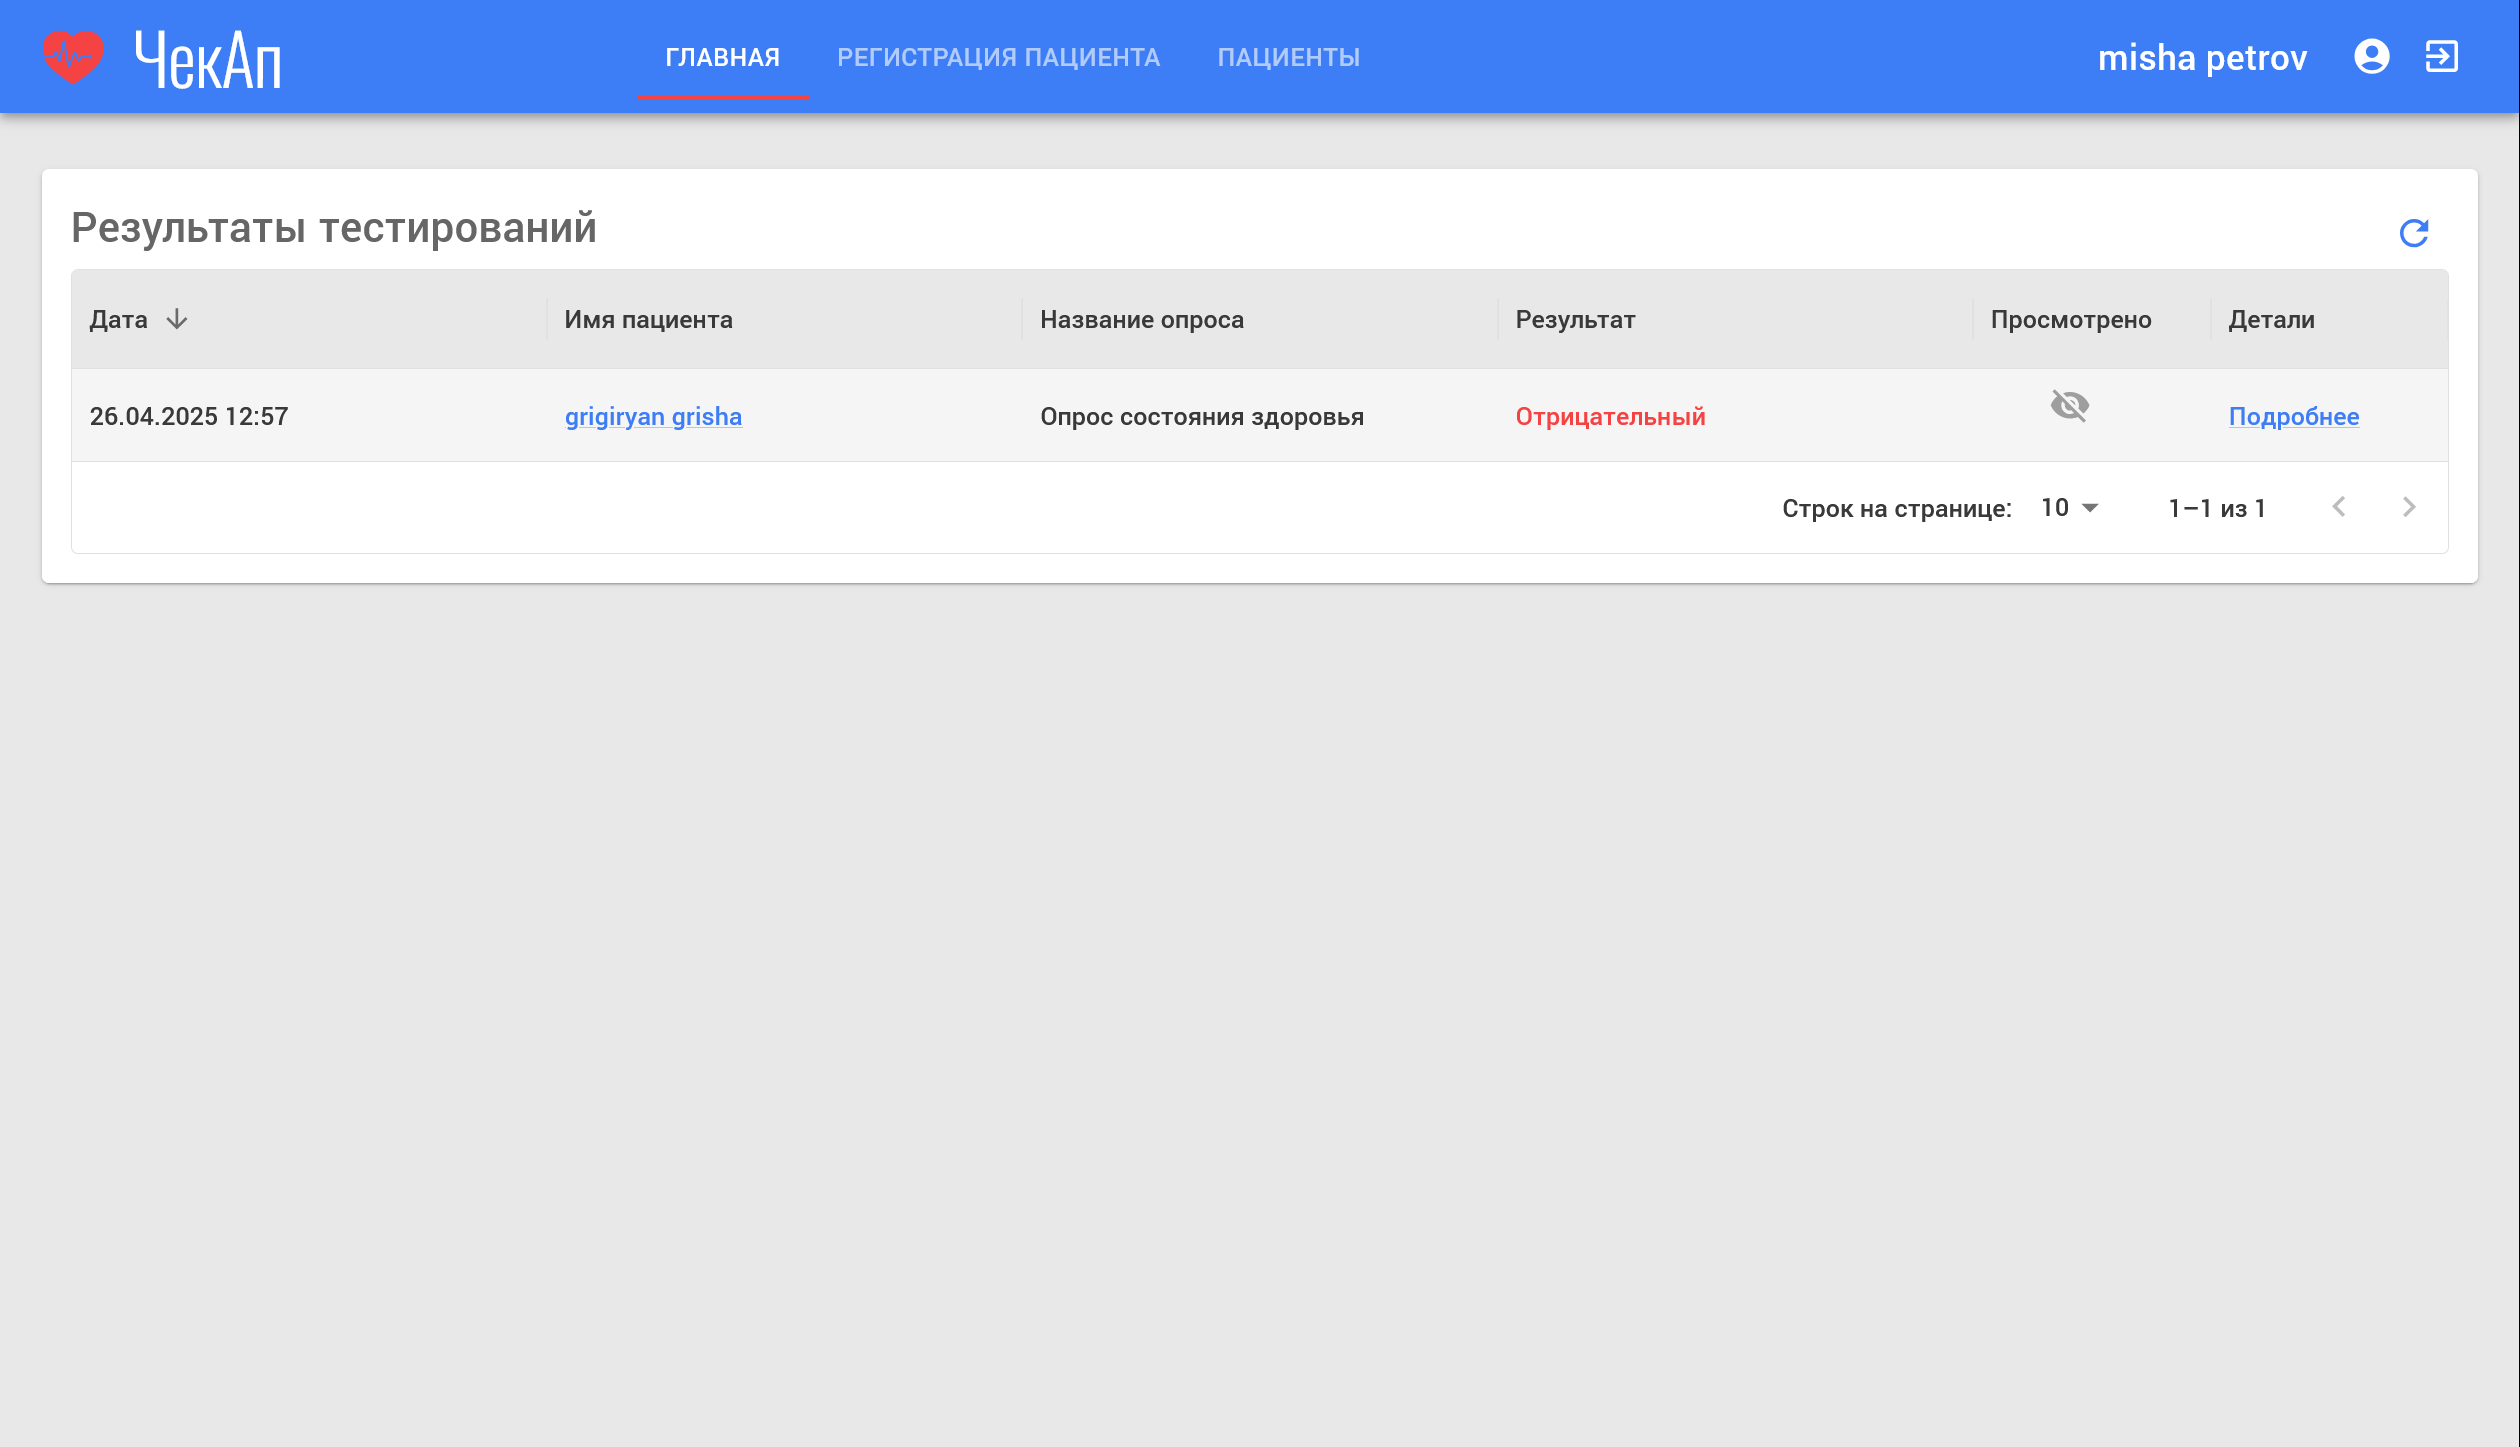
\includegraphics[scale=0.17]{images/screenshots/main_page}
        \caption{Главная страница.}\label{fig:figure5}
    \end{figure}

    \subsection{Опрос}\label{subsec:2}
    На страницу с конкретным прошедшим опросом можно перейти по ссылке из главной страницы.
    Здесь представлено подробно о пациенте и конкретные вопросы и ответы для более возможности оценки ответов лично врачом.
    \begin{figure}[ht]
        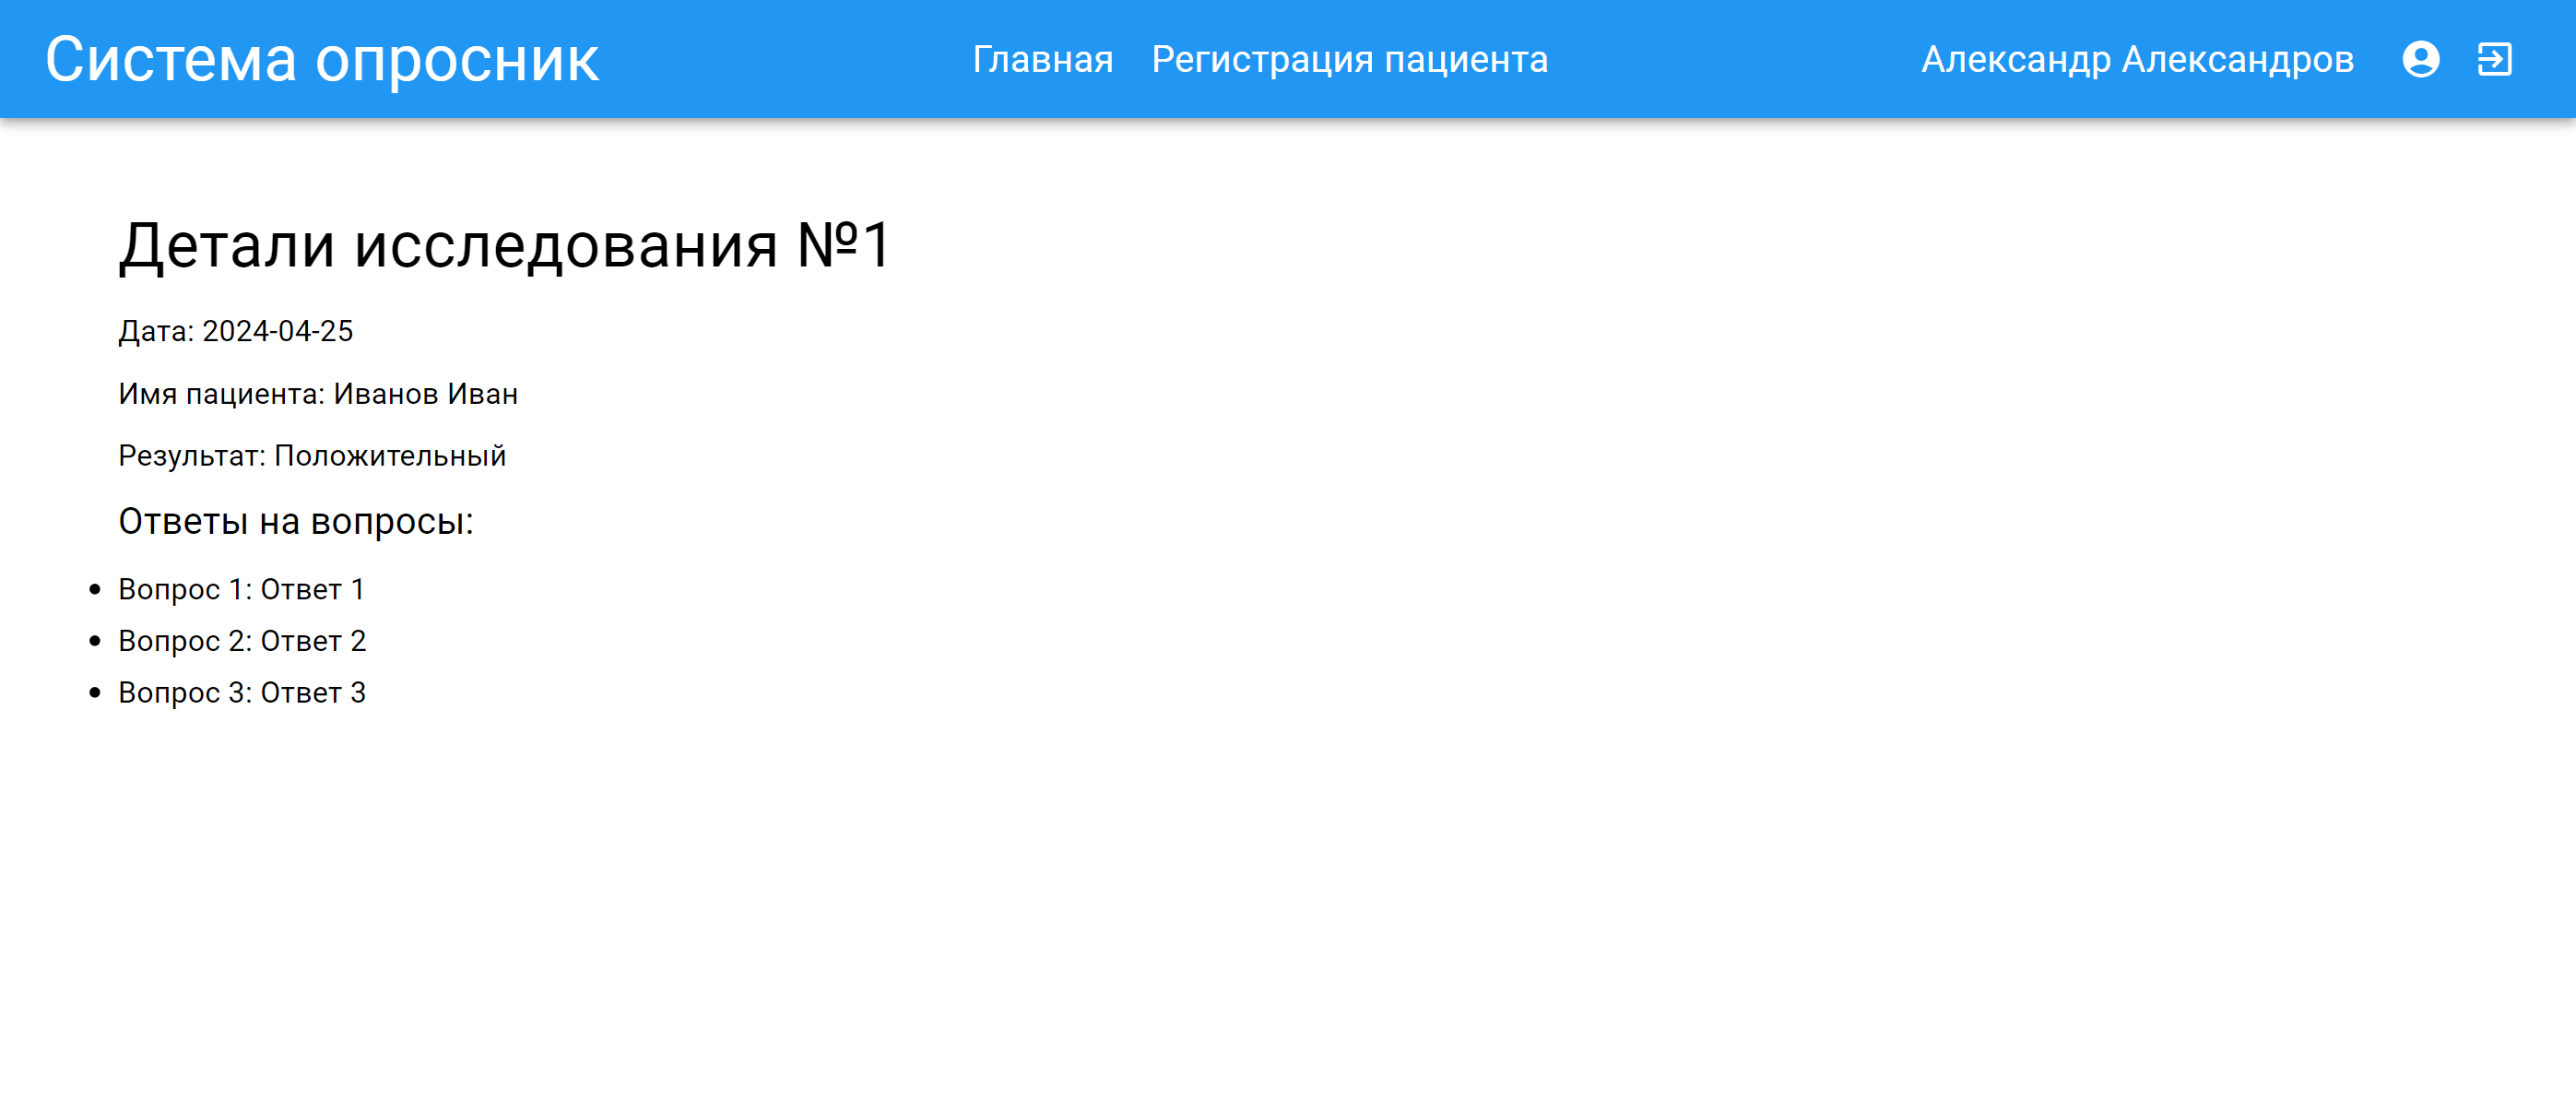
\includegraphics[scale=0.17]{images/screenshots/inquirer}
        \caption{Представление ответов в опросе.}\label{fig:figure6}
    \end{figure}

    \newpage
    \subsection{Регистрация пациента}\label{subsec:-3}
    На этой странице представлена форма для регистрации нового пациента (см.\ рис~\ref{fig:figure7})
    \begin{figure}[ht]
        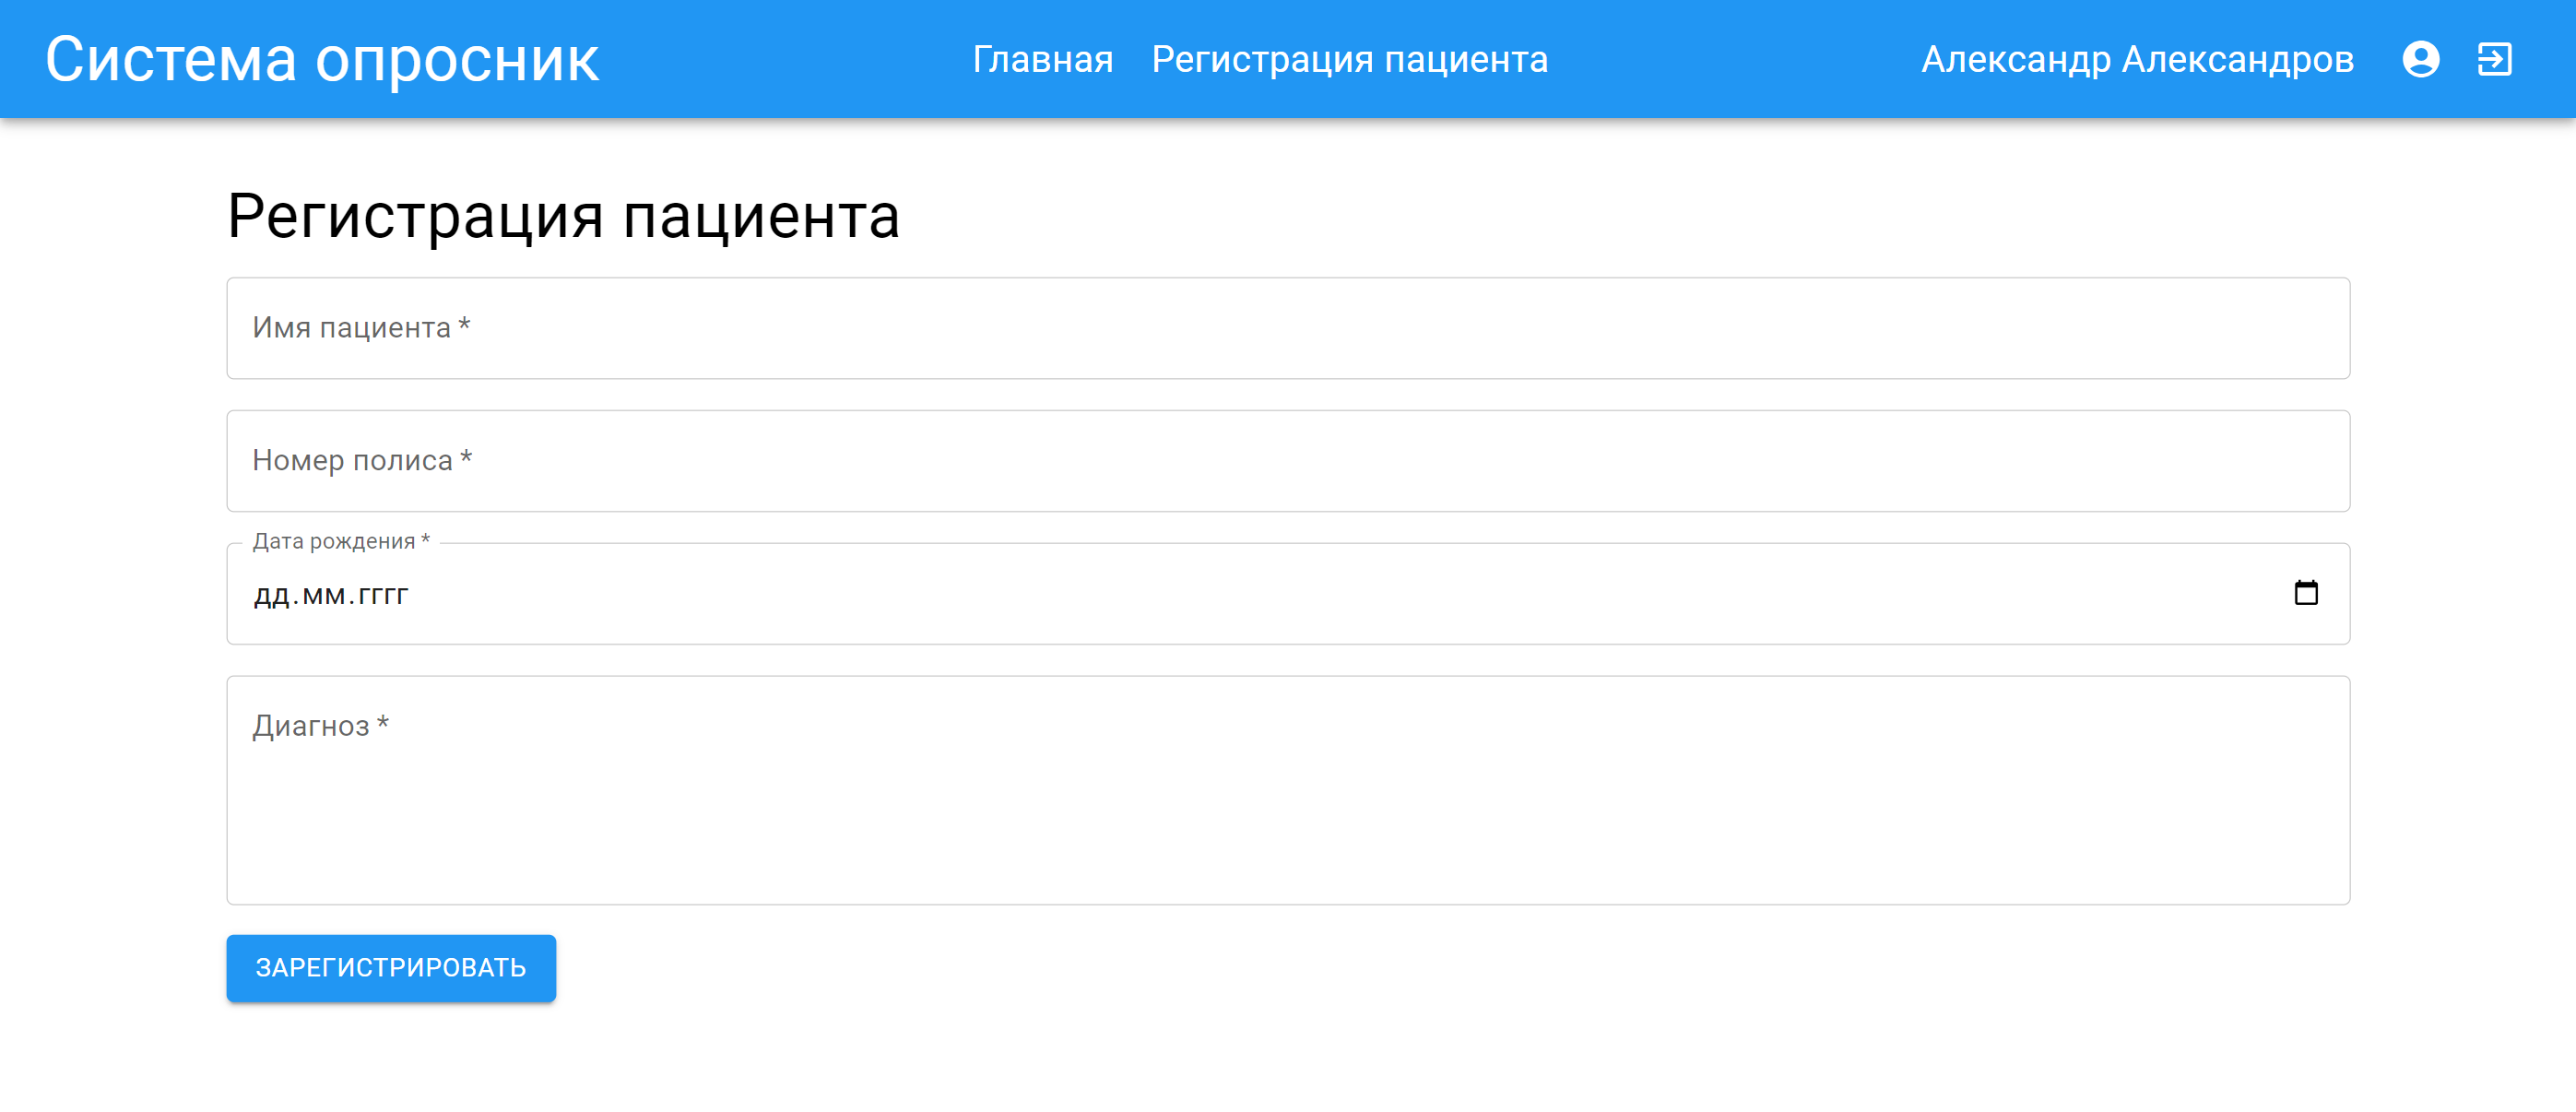
\includegraphics[scale=0.17]{images/screenshots/registration}
        \caption{Форма регистрации пациента.}\label{fig:figure7}
    \end{figure}

    \newpage
    \section*{Заключение}
    \addcontentsline{toc}{section}{Заключение}
    \label{sec:3}
    В ходе выполнения были изучены и определены основные технологии, которые будут использоваться в проекте.
    В этом семестре сервер и веб-приложение разрабатывались отдельно, начала прорабатываться архитектура взаимодействия.
    Основные экраны приложения отрисованы.
    На данном этапе приложение использует mock-данные для демонстрации интерфейса.

    Основные цели на дальнейшую разработку:

    \begin{itemize}
        \item Связать приложение с сервером.

        \item Более подробно проработать UI и UX приложения.

        \item Разработать страницу, на которой будет происходить создание новых опросов.

        \item Адаптировать верстку под мобильные устройства.

    \end{itemize}

    Ссылка на проект Github:
    \url{https://github.com/miharbm/sechenovinquier.git}


    \newpage
    \addcontentsline{toc}{section}{Список литературы}
    \begin{thebibliography}{99}

        \bibitem{borgoyakov2016} Боргояков Е.\,А., Кособрюхова О.\,В. Современные подходы в профилактике неинфекционных заболеваний.\ — Ачинск: Изд-во Ачинского гос.\ пед.\ университета, 2016.\ — 150 с.

        \bibitem{banks2020} Banks, A., Porcello, E. Learning React: Modern Patterns for Developing React Apps.\ — O'Reilly Media, 2020.\ — 350 p.\ ISBN 978--1492051725.

        \bibitem{stefanov2016} Stefanov, S. React - Up \&Running: Building Web Applications.\ — O'Reilly Media, 2016.\ — 280 p.\ ISBN 978--1491931820.

        \bibitem{wieruch2023} Wieruch, R. The Road to React: Your Journey to Master React.js in JavaScript (2023 Edition).\ — Independently published, 2023.\ — 380 p.\ ISBN 978--1730853937.

        \bibitem{copes2021} Copes, F. Vite Handbook: Getting Started with Vite.js.\ — Independently published, 2021.\ — 220 p.\ ISBN 979--8728328575.

        \bibitem{boduch2019} Boduch, A. React Material-UI Cookbook.\ — Packt Publishing, 2019.\ — 300 p.\ ISBN 978--1789616111.

    \end{thebibliography}


\end{document}